\documentclass[
    paper=a4,
    % fontsize=12pt,
    div=calc,
    numbers=noendperiod,
    % twocolumn,
]{scrartcl}

\usepackage[utf8]{inputenc}
\usepackage[T1]{fontenc}
\usepackage[ngerman]{babel}

\usepackage{microtype}
\usepackage{libertine}
\usepackage[libertine]{newtxmath}
\usepackage[headsepline]{scrlayer-scrpage}

\usepackage{booktabs}
\usepackage{siunitx}
\usepackage{pdfpages}
\usepackage{enumitem}

\usepackage{flushend}

\usepackage[
    bookmarksnumbered   =   true,
    breaklinks          =   true,
    colorlinks          =   true,
    pdftitle            =   {Mentoring Jan Hoegen},
    pdfsubject          =   {Mentoring HKA WS 22/23},    
    pdfauthor           =   {Jan Hoegen},
]{hyperref}

\titlehead{Hochschule Karlsruhe\\Univerity of Applied Sciences}
\subject{Studiengang Elektro- und Informationstechnik}
\title{Mentoringbericht Wintersemster 2022/23}
% \subtitle{Wintersemster}
\author{Jan Hoegen\\\href{mailto:jan.hoegen@web.de}{jan.hoegen@web.de}}
\date{Erstellt am \today}
% \publishers{xx}

\ihead{Jan Hoegen}
\chead{Mentoringbericht WS 22/23}
\ohead{\today}

\newcommand{\legend}[1]{\par\footnotesize\textbf{Legende}: #1\par}
\newcommand{\gquotes}[1]{\glqq #1\grqq}
\newcommand{\shadowsection}[1]{%
    \refstepcounter{section}
    \addcontentsline{toc}{section}{\protect\numberline{\thesection}{#1}}
}

% \flushend
\flushbottom

\begin{document}

\maketitle

\tableofcontents

\section{Rahmenbedingungen}
    Das Mentoringprogramm richtet sich an Erstsemesterstudentinnen und -Studenten an der Hochschule Karlsruhe im Studiengang Elektro- und Informationstechnik für das Wintersemster 2022/23. Organisiert wird es vom Zentrum für Lehrinnovation der HKA. Ziel ist es, den Studierenden den Einstieg ins Studium durch erfahrene Kommilitonen zu erleichtern.

    Ich bin 23 Jahre alt, studiere Elektro- und Informationstechnik im zweiten Bachelorsemester, und nehme zum ersten Mal als Mentor an diesem Programm teil. Gemeinsam mit Raphael Hansjosten (7. Bachelorsemester) bilden wir ein Team und betreuen insgesamt elf Mentees. 

    \subsection*{Vorkenntnisse}
        Raphael Hansjosten nimmt zum zweiten Mal als Mentor teil und studiert bereits seit 3 Jahren an der Hochschule, daher kann ich auf seinen großen Erfahrungsschatz und sein hochschulspezifisches Wissen zurückgreifen. 

        Obwohl ich über weniger Erfahrung über das Studium an der HKA verfüge, fühle ich mich dennoch gut vorbereitet, die Mentees in ihrem ersten Semester zu unterstützen. Dank meiner Vorkenntnisse als lizenzierter C-Trainer im Bereich Leistungssport Erwachsene Volleyball bin ich mit den Themen Mehrjahreszielsetzung, Planung und Umsetzung, sowie Wissensvermittlung gegenüber Jugendlicher geübt.  
        Aufgrund meiner Werkstudententätigkeit im Rettungsdienst und Krankentransport Karlsruhe bin ich über psychische Probleme, Stresssituationen      und ihre Anlaufstellen zur Selbsthilfe sensibilisiert.  
 
\section{Zielsetzung}
    \label{sec:ziele}
    Folgende Aufgaben wurden an die Mentoren formuliert:

    \begin{itemize}[noitemsep]
        \item Beratung der Mentees über das erste Semester hinweg geben
        \item Anlaufstelle für Fragen rund um das Studium sein
        \item Wissen und Erfahrung teilen
        \item Fachliche und organisatorische Tipps geben
        \item Mentees motivieren, Entscheidungen eigenständig und reflektiert zu treffen
        \item Netzwerke für Mentees schaffen
        \item Feedback geben
    \end{itemize}

    Daraus entwickelten Raphael und ich folgende Ziele und einige Beispiele für unsere Mentoringarbeit:

    \subparagraph{Hilfe beim Ankommen und Zurechtfinden im Studium:}
        Zugang zur Prüfungsanmeldung, Zugang zu Fachschaftsdokumenten, Lerngruppen finden, Anmeldung zum Hochschulsport, \dots

    \subparagraph{Probleme vorbeugen und Hilfestellung geben:}
        Tipps zum Schieben von Klausuren, Anpassung von Semesterzielen und Wochenlernplänen, Möglichkeiten zur Selbsthilfe bei psychischen Problemen, \dots

    \subparagraph{Relevante Informationen und Tipps weitergeben:}
        effektive Lernmethoden, Tipps zur guten Klausurvorbereitung, Vorlesungen priorisieren und effektiv mitarbeiten, \dots

\section{Bericht und Reflexion der Mentoringtreffen}
    Im Folgenden werden die einzelnen Treffen beschrieben und von mir reflektiert. Unterlagen zur Vor- und Nachbereitung der Treffen finden sich im Anhang \ref{app:orga}. 

    \subsection{Online-Treffen am 29. September 2022}
        Das online-get-together dauerte ca. \SI{30}{\minute}. Ich führte eine kurze Vorstellungsrunde mit den initial drei teilnehmenden Mentees durch und erklärte, dass ich das Mentoring im Tandem mit Raphael Hansjosten führen werde. Während eine Whatsappgruppe mit allen Teilnehmer*innen erstellt wurde und die Mentees bereits an der ersten Terminumfrage teilnahmen, kamen weitere Erstsemesterstudierende dem Meeting hinzu. Somit stieg die Gesamtteilnehmerzahl von Raphael und mir auf insgesamt elf.

        Mein Vorgehen, bereits während des Matchings die Teilnehmer eine Terminumfrage für das nächste Treffen durchführen zu lassen, funktionierte wie erwartet sehr gut und führte zu einer hohen Beteiligung. Ich war mir sicher, dass ich mit der doppelten Gruppengröße gut umgehen kann.

    \subsection{Offline-Treffen am 4. Oktober 2022}
        Das erste Offline-Treffen fand im Fachschaftsraum EIT statt und ging \SI{120}{\min}. Hier konnten wir uns gegenseitig besser kennelernen und uns über Gesprächsthemen für die zukünftigen Treffen austauschen. Das alles fand im Rahmen eines von der Fachschaft organisierten Grillabends statt. Leider konnte Raphael krankheitsbedingt nicht teilnehmen. Zusätzlich lernten die Mentees die Fachschaft mit all ihren Vorteilen, ihren Mitgliedern und weiteren EIT-Studierenden kennen.

        An dieser Stelle kamen bereits einige Fragen zum Angebot \gquotes{erfolgreich starten} der HKA und ich konnte mein persönliche Einschätzung wiedergeben. Außerdem konnte ich meine Mentees besser kennen lernen und das Eis brechen.

    \subsection{Offline-Treffen am 18. Oktober 2022}
        Dieses Treffen wurde zusammen mit einer weiteren EIT-Mentoren-Gruppe durchgeführt und wurde in zwei Teile geteilt: Im ersten Teil hielten wir Mentoren einen Vortrag zum Thema \gquotes{Organisation von Vorlesungen} über \SI{60}{\min}. Die von mir erstellten Notizen und das Handout finden sich im Anhang \ref{app:meeting3}. Den zweiten Teil des Abends verbrachten wir ca. \SI{330}{\min} in einer Bowlingbahn in Karlsruhe. Jedoch blieben nicht alle Mentees solange, sondern beendeten den Abend zu verschiedenen Zeitpunkten

        Während dem Vortrag konnte ich auf Themen wie sinnvolle Zielsetzung für das Semester, Erarbeitung von Teilzielen und deren Planung eingehen. Außerdem konnten die Mentoren ihre eigenen Erfahrungen und Empfehlungen abgeben, wie man Vorlesungen am besten vor- und nachbereitet. Es wurden darüber hinaus Hinweise zur Fachschaft und anderen Diensten für Studierende in Karlsruhe gegeben.

        An der Bowlingbahn konnten wir uns mit den Mentees über die vorherigen Punkte weiter austauschen und Hilfestellung zu verschiedenen Themen geben. 

    \subsection{Offline-Treffen am 9. November 2022}
        Während der Mittagspause veranstalteten Raphael und ich eine Gesprächsrunde für ca. \SI{60}{\min}. Mit drei teilnehmenden Mentees sprachen wir über die Themen aus dem letzten Treffen, unsere Erfahrung mit verschiedenen Dozenten, Prüfungen und unsere Freizeit.
        
        Aufgrund der geringen Teilnehmerzahl hatte das Treffen eine lockere Atmosphäre.

    \subsection{Offline-Treffen am 29. November 2022}
        An diesem Treffen schloss sich uns erneut eine Tandem-Mentoren-Gruppe an, um die anwesenden Mentees auf ihre bevorstehende Klausurenphase vorzubereiten. Die Veranstaltung ging \SI{90}{\min} und fand abends in einem leeren Hörsaal statt. In dieser Zeit sorgten wir dafür, dass jeder Mentee erfolgreich mit einer TAN seine Prüfungsanmeldung einsehen konnte und behandelten anschließend die Themen Lernplanerstellung, Klausurvorbereitung und den Umgang mit Lernstress. Meine Unterlagen zur Vorbereitung, Präsentation und Handout finden sich im Anhang \ref{app:meeting4}.

        Meiner Meinung nach konnten hier die Informationen weitergegeben werden, die den Mentees langfristig am weitreichendsten helfen werden. Ich zeigte ihnen auf, dass sie noch acht Wochen bis Klausurbeginn haben und bereits seit zwei Wochen auf die Klausuren lernen sollten. Des Weiteren konnte ich einige Grundgedanken aus der Trainingslehre in das Studium übertragen: 
        
        Das Semesterziel der meisten Studenten ist es, die Klausuren zu bestehen. Abhängig von der Anzahl und Art der Klausuren ist eine umfangreiche Vorbereitung und Training notwendig. Um dies zu erreichen, wird das Problem in Teilgebiete unterteilt und diese nacheinander bearbeitet. Dazu müssen realistische Zwischenziele gesetzt werden und das Handeln muss stets auf die Zwischenziele ausgerichtet sein. Falls abzusehen ist, dass gewisse Ziele nicht erreicht werden können, müssen die Ziele angepasst und z.B. eine Klausur geschoben werden. je näher man dem Semesterende kommt und alle Teilgebiete erlernt hat, desto wichtiger wird es, möglichst prüfungsnah zu üben. Dies beinhaltet Umfang, Zeitdruck, äußere Umgebung, Tageszeit, genutzte Hilfsmittel \dots

        Darüber hinaus sprach ich das Thema Lernstress und psychische Erkrankungen grundlegend an. Auch an dieser Stelle haben die anderen Mentoren von eigenen Erfahrungen berichtet und eigene Tipps gegeben.

    \subsection{Offline-Treffen am 21. Dezember 2022}
        Raphael Hansjosten organisierte ein Vorstellungsrunde mit anschließender Fragerunde in Kleingruppen über die Vertiefungsrichtungen unseres Studiengangs über \SI{60}{min}. Er gab allen Studenten im Grundstudium -- egal ob Mentee oder nicht -- die Gelegenheit, von Kommilitonen Eindrücke über die Vertiefungsfächer zu erhalten. Auch ich konnte von dieser Veranstaltung profitieren. Dafür danke ich ihm sehr.

\section{Ausblick}
    In der Zukunft sind zwei weitere Treffen geplant, ihr Inhalt und der geplante Zeitraum werden nun kurz skizziert.

    \subsection{Geplantes Treffen im Januar 2023}
        Das vorletzte Mentoringtreffen wird kurz vor der Prüfungsphase stattfinden. Vermutlich wird es hauptsächlich darum gehen, die Sorgen der Mentees zu beseitigen und Hilfestellung bei Frust, Unsicherheit und Überforderung zu geben. 
        
        Doch ich bin mir sicher, dass wir unsere Mentee gut auf diese Zeit vorbereitet haben und sie diese Phase meistern werden. Viele von ihnen sind engagiert in der Fachschaft oder anderen Bereichen der Hochschule und die meisten wirken auf mich um ihr Studium äußerst motiviert.

    \subsection{Geplantes Treffen im Februar 2023}
        Abschließend wird es im Februar ein Reflexionsgespräch zwischen den Mentees, Raphael und mir geben. Womöglich wird auch das Ende der ersten Klausurenphase ein wenig gefeiert. Und auch an dieser Stelle können Raphael und ich Hilfestellung geben, wenn ein Mentee beispielsweise eine Klausur nicht bestanden hat. 
        
        Ich bin bereits gespannt darauf, ihr ehrliches Feedback zu hören und zu erfahren, ob unsere Mentoringarbeit einen spürbaren Einfluss auf sie hatte. Damit ich dann meinen Anteil der Mentoringtreffen besser reflektieren und meine Mentoringarbeit verbessern. Falls ich im nächsten Semester erneut Mentor sein möchte, wäre dies äußerst hilfreich für mich und meine zukünftigen Mentees. 
        
\section{Abschließende Reflexion}
    In Tabelle \ref{tab:time} sind die einzelnen Mentoringtreffen und die Gesamtdauer aufgelistet. Es ist zu erkennen, dass Raphael und ich beinahe \SI{5}{\hour} mehr Mentoringarbeit geleistet haben, als gefordert war -- Vor- und Nachbereitung nicht mitberechnet. 

    \begin{table}[htb]
        \centering
        \caption{Dauer der Mentorentreffen}
        \label{tab:time}
        \begin{tabular}{lcr}\toprule
            Treffen &   Datum           &   Zeit\\\midrule
            1       &   29.09.2022      &   \SI{30}{\minute}\\
            2       &   04.10.2022      &   \SI{120}{\minute}\\
            3       &   18.10.2022      &   \SI{390}{\minute}\\
            4       &   09.11.2022      &   \SI{60}{\minute}\\
            5       &   29.11.2022      &   \SI{90}{\minute}\\
            6       &   21.12.2022      &   \SI{60}{\minute}\\
            7       &   (20.01.2023)    &   \SI{60}{\minute}\\
            8       &   (10.02.2023)    &   \SI{60}{\minute}\\
            \addlinespace
            \multicolumn{2}{l}{gesamt}  &   \SI{870}{\minute}\\\bottomrule
        \end{tabular}
        \vspace{0.5em}
        \legend{Die letzten beiden Treffen haben noch nicht stattgefunden und sind daher als Richtwert anzusehen.}
    \end{table}

    An den Treffen waren durchschnittlich neun bis elf Mentees anwesend, ausgenommen Treffen 4. Als wir uns mit zwei weiteren Mentoren zusammen geschlossen haben, waren beinahe 20 Erstsemesterstudierende da. Ich denke, dass die Mentees sehr davon profitiert haben, dass die Gruppen für zwei Treffen zusammengelegt wurden. Sie erhielten die Informationen gebündelt und erfuhren die Ansichten von vier verschiedenen Mentoren. 

    Insgesamt hat mir die Mentoringarbeit viel Freude bereitet. Aufgrund meiner außerstudentischen Erfahrung viel es mir leicht, die Treffen vorzubereiten und zu organisieren. Die Zusammenarbeit mit Raphael verlief außerordentlich gut, er leistete einen großen Beitrag zu unserer Mentorenarbeit.

    Über das Semester hinweg wurden die Mentees aufgeschlossener und stellten immer mehr Fragen an uns. Vereinzelt wurde auch bereits Feedback geäußert: die Mentees würden merken, wie viel Aufwand und Gedanken wir uns über die Mentoringtreffen machen. Wir würden uns richtig Mühe geben. Ein Mentee sagte mir, sie sei froh, dass ich ihr Mentor bin. Ein anderer teilte mir mit, dass die Mentoringtreffen und unser Auftreten ihn sehr motivieren. 

    Es war toll zu sehen, wie sich unsere Erstsemesterstudent*innen einleben. Die Mehrheit unserer Mentees ist inzwischen in der fachschaft aktiv und vernetzt sich mit Studierenden aus allen Semestern. Ich habe fest vor, mit meinen Mentees und mit Raphael regelmäßig in Kontakt zu bleiben. Ich hoffe darauf, dass möglichst viele von ihnen ihr Studium fortsetzen werden.

    % \pagebreak

    \subsection*{Nutzung der Checkliste}
        Die Checkliste wurde nur in geringen Umfang dazu genutzt, die Mentoringtreffen vorzubereiten. Stattdessen stützten Raphael und ich auf unsere eigenen Erfahrung und Grundgedanken. An dieser Stelle waren die Ziele, die in Abschnitt \ref{sec:ziele} beschrieben werden, sehr hilfreich und eine gute Orientierung. Ich würde mir wünschen, dass einige Punkte aus unseren Handouts mit in die Checkliste fließen und damit zukünftigen Mentoren helfen.  

\appendix
\clearpage

    \shadowsection{Unterlagen Organisation der Mentoringtreffen}
        \label{app:orga}
        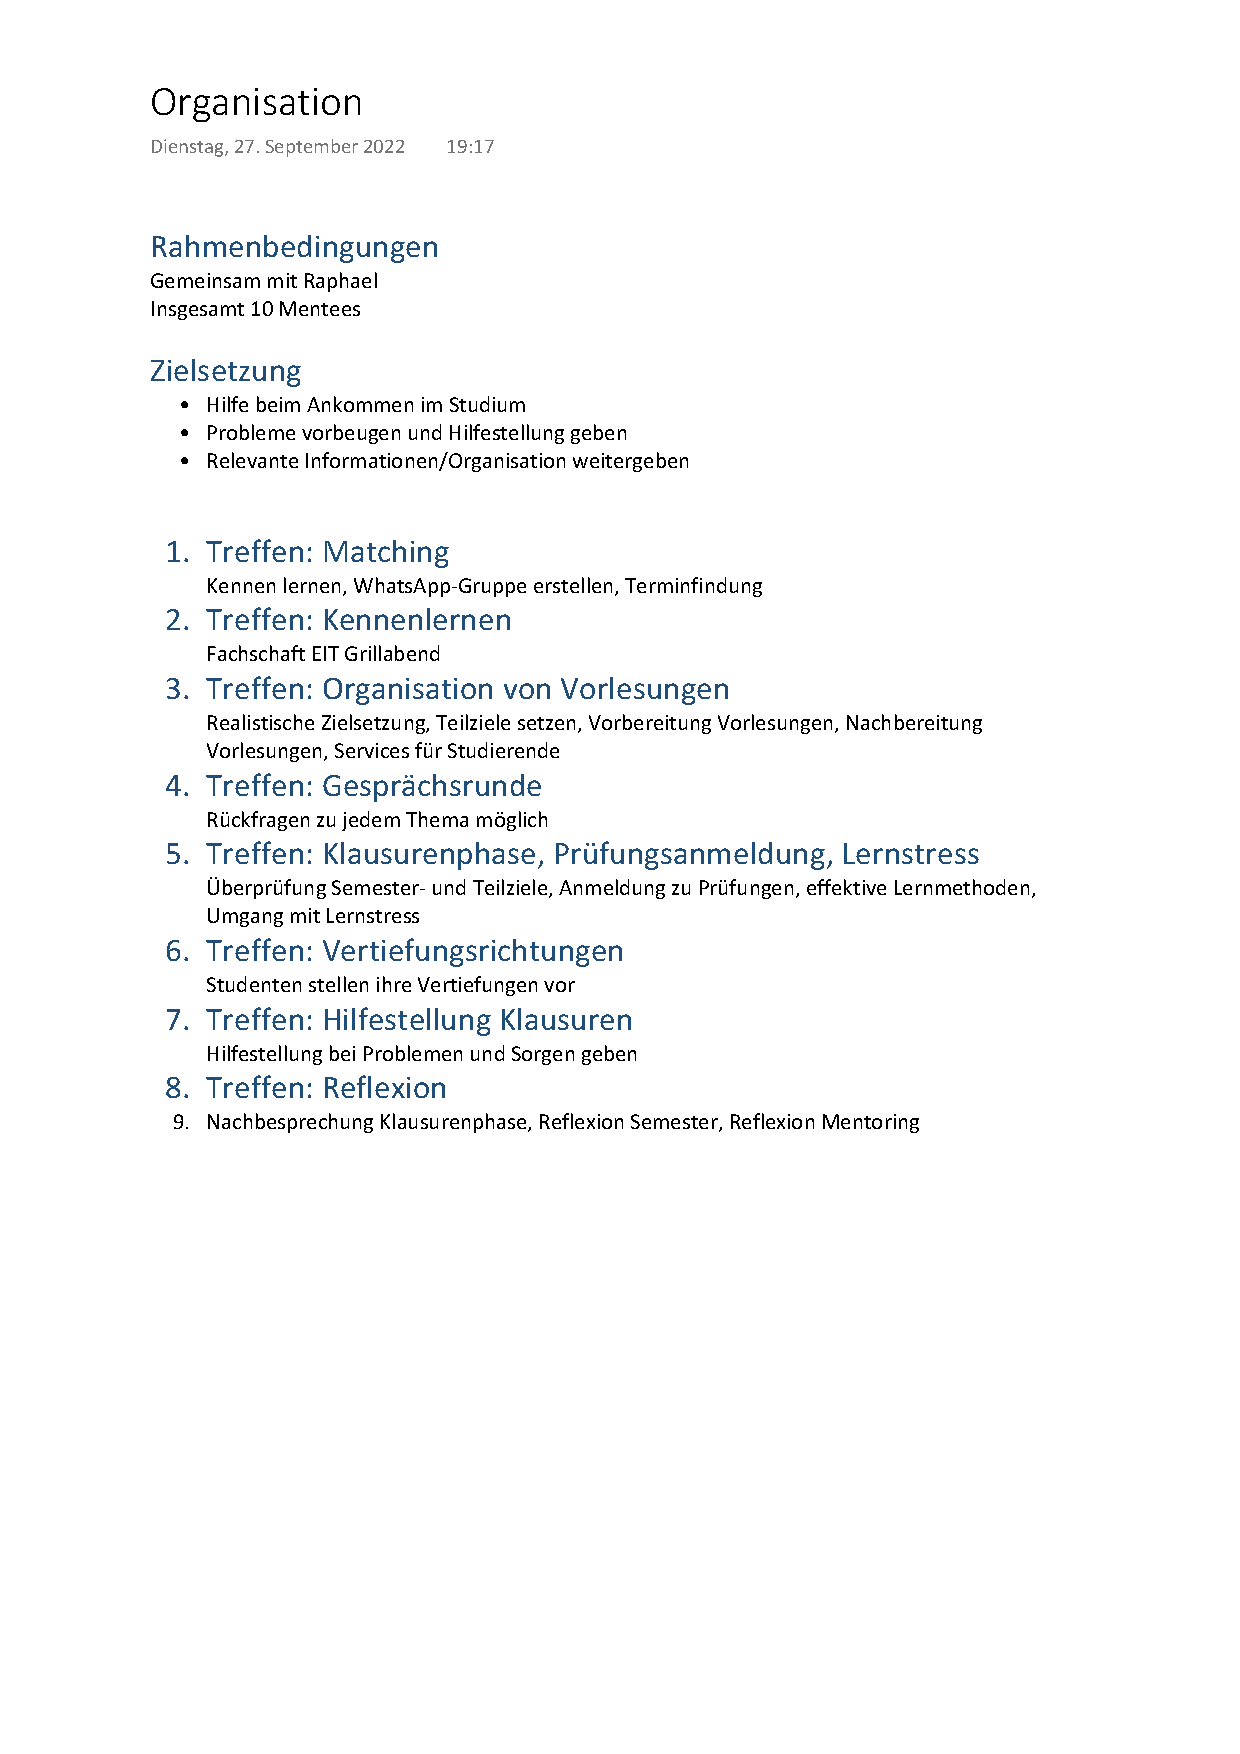
\includepdf[]{notizen-orga.pdf}

    \shadowsection{Handout Treffen 3}
        \label{app:meeting3}
        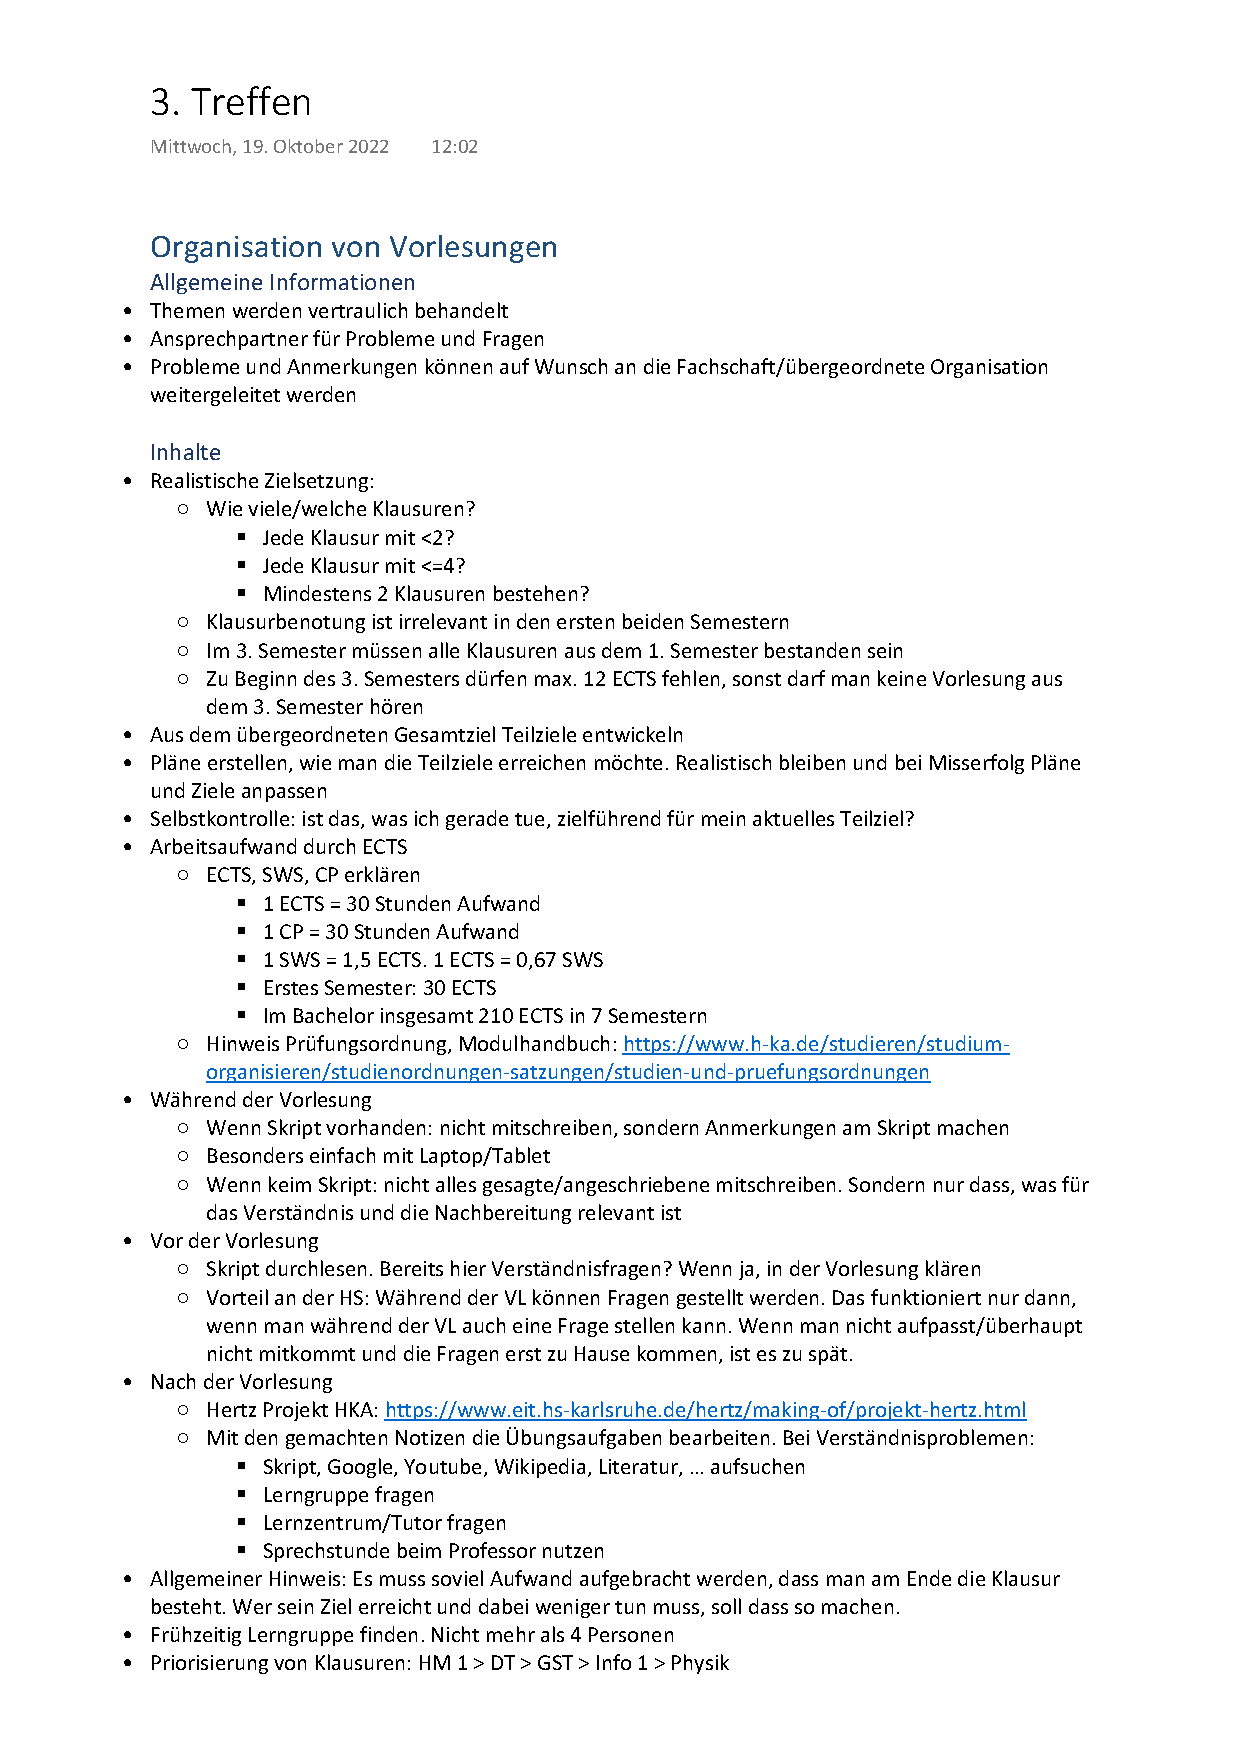
\includepdf[pages={1-2}]{treffen-3-ws22.pdf}

    \shadowsection{Handout Treffen 4}
        \label{app:meeting4}
        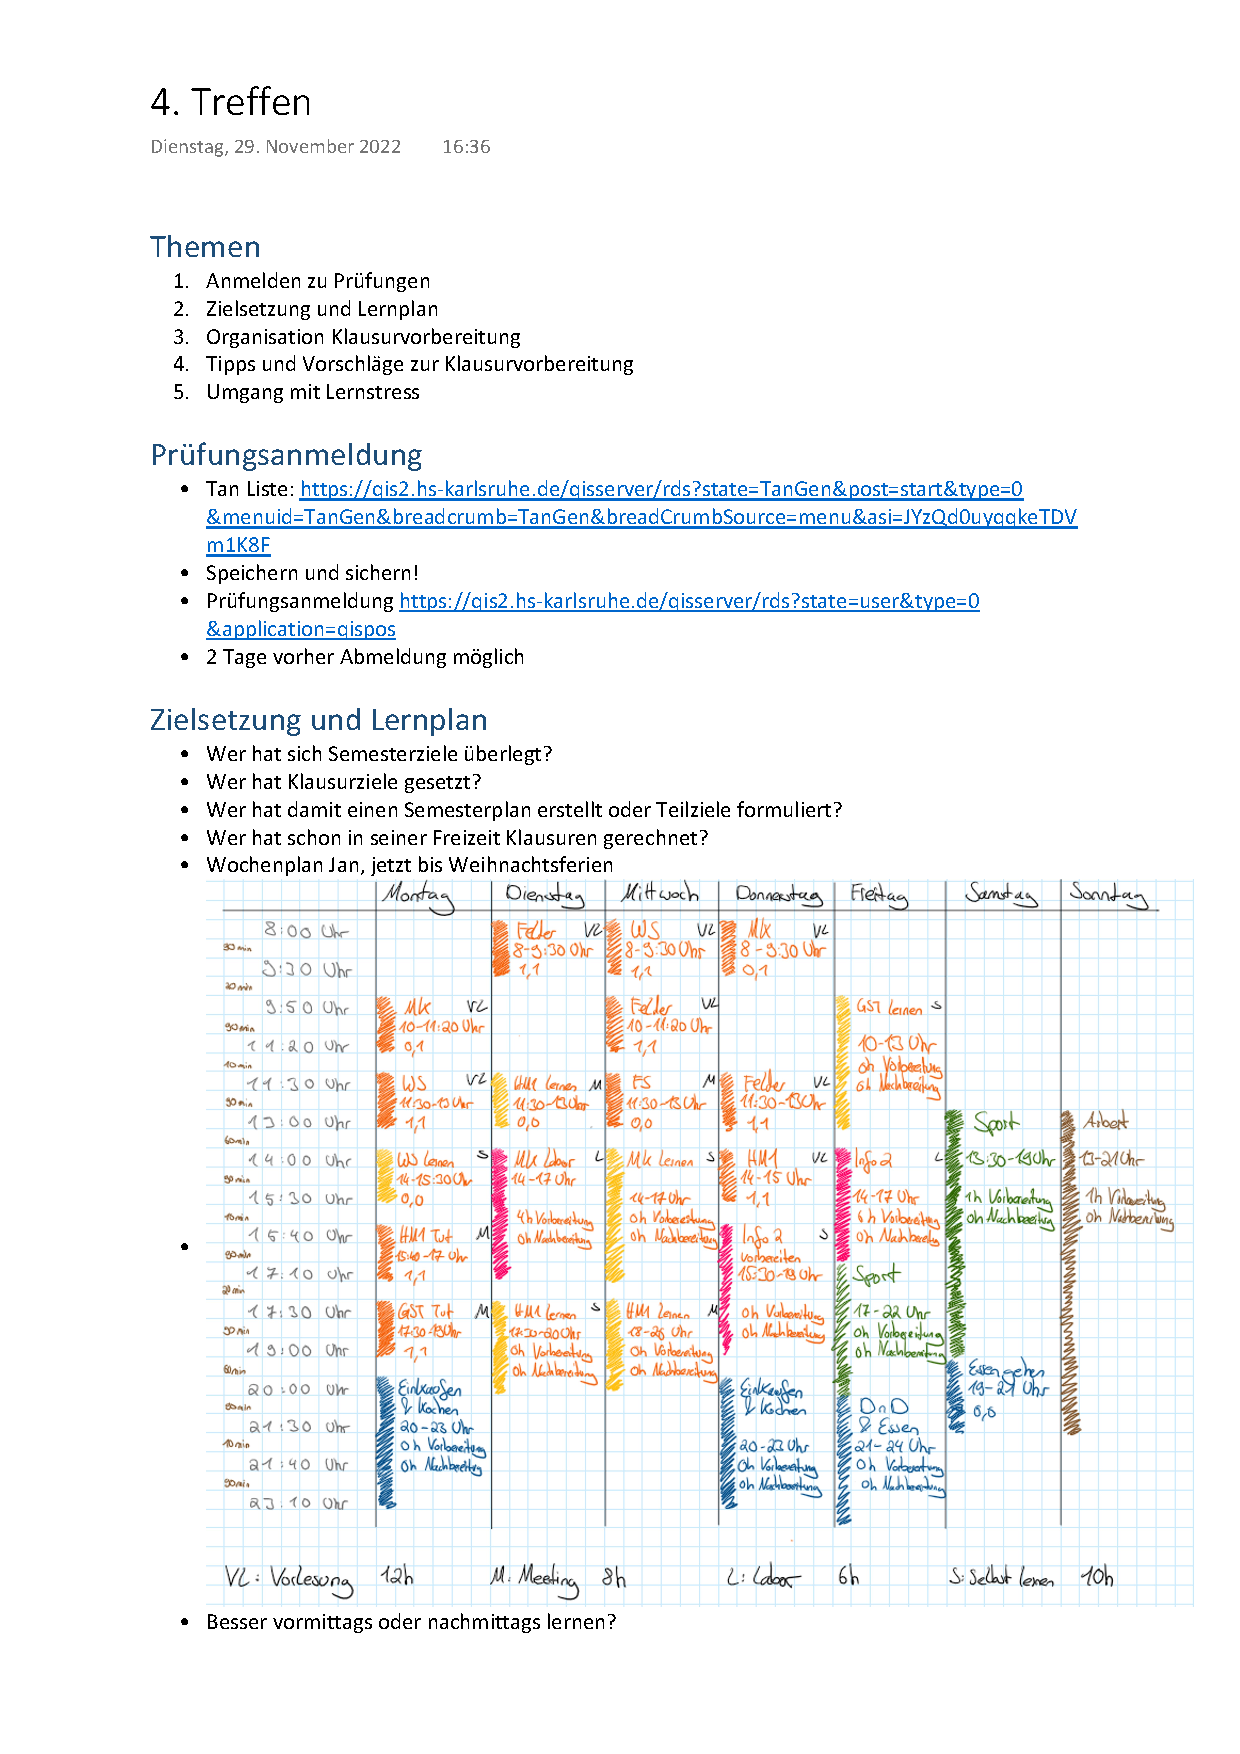
\includepdf[pages={1-3}]{treffen-4-ws22.pdf}

\end{document}